\documentclass{article}
\usepackage{geometry}
\usepackage{amsmath}
\usepackage{graphicx}
\usepackage{enumitem}
\usepackage{bm}
\usepackage{float}
\usepackage{accents}
\usepackage{undertilde}

% added this to stop hbadness warning
\hbadness = 5000000

\geometry
{
	headheight = 4ex,
	includehead,
	includefoot,
	paper = a4paper,
	inner = 2.5cm,
	outer = 2.5cm,
	bindingoffset = 0.5cm,
	top = 2cm,
	bottom = 1.5cm
}


\title{\Huge Problem Set 3} 
\vspace{1cm}
\author {\Large Chara Tsirka 03315, Prodromos Avramidis 03291}

\begin{document}

\maketitle
\begin{center}
\vspace{1cm}

\includegraphics[width=0.3\textwidth]{uthlogo.png}
\vspace{2cm}
\end{center}
\begin{center}
  \Huge Neurofuzzy Computing \vspace{1cm}

  \Large Fall Semester 2023-2024 \vspace{1cm}

  \Large Professor: Dimitrios Katsaros
\end{center}


%Problem 1
\newpage
\noindent \textbf{Problem 1}

\noindent Design by hand (i.e., select manually the layers, the number of neurons per layer, the 
weights and biases per layers) an RBF network to perform the classification illustrated in 
the following figure. The network should produce a positive output whenever the input 
vector is in the shaded region and a negative output otherwise. Provide arguments for the 
selection of weights and biases
\begin{center}    
    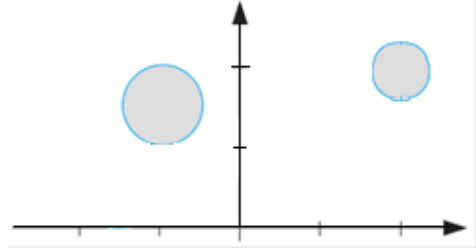
\includegraphics[width=0.4\textwidth]{pr1.png}
    \vspace{2cm}
\end{center}



\noindent \underline{\textbf{\textit{Solution:}}}

\noindent From the problem statement we know that the RBF network will have two inputs and one output.
We will use two neurons in the first layer because we have 2 shaded regions. 
The rows of the first layer weight matrix
will create the centers for the two basis functions so that we can produce the maximum outputs there. 
As we can see in the figure the center for the first shaded region
is (-1, 1.5) and the center for the second shaded region is (2,2) so the first layer weights matrix will be: \\
\begin{center}
  
$ W^1 = \begin{bmatrix}
  - 1 & 1.5 \\
  2 & 2
\end{bmatrix} $
\end{center}

\noindent Now we need to choose the biases for the first layer. We see in the figure that the radius of the first 
region is approximately 0.5 and the radius of the second region is approximately 0.25. 
Because the first region is wider than the second region the first bias will be smaller than the second bias.
If we choose biases 1 and 2 respectively we get:
$a = e^{-n^2}= e^{-(1*0.5)^2} \approx 0.18$ and $a = e^{-n^2}= e^{-(2*0.25)^2} \approx 0.18$
Therefore, each basis function will have a peak of 1 at the centers, and will drop to 0.18 at the edge of the regions.
So the first layer bias will be:
\begin{center}
  
  $ b^1 = \begin{bmatrix}
    1 \\
    2 
  \end{bmatrix} $
  \end{center}

  \noindent We want the output to be negative for inputs outside the shaded regions,
  so we will use a bias of -1 for the second layer, and we will use a value of 2
  for the second layer weights, in order to bring the peaks back up to 1. The second layer weights and bias are:

  \begin{center}
  
    $ W^2 = \begin{bmatrix}
      2 & 2
    \end{bmatrix},
     $
    $ b^2 = \begin{bmatrix}
      -1
    \end{bmatrix} $

    \end{center}
  
  



%Problem 2
\newpage
\noindent \textbf{Problem 2}

\noindent Write a MATLAB/python/… program to implement the steepest descent algorithm for the $ 1-S^1-1$ RBF network. 
Train the network to approximate the function:
\begin{center}
    $g(p) = 1 +sin(p*\pi/8) for -4 \leq p \leq 4$.    
\end{center}  

\begin{itemize}
    \item To train the network, select 30 data points at random from the interval $-4 \leq p \leq 4$.
    \item Initialize all parameters (weights and biases in both layers) as small random numbers, 
    and then train the network to convergence. (Experiment with the learning rate $\alpha$, to 
    determine a stable value.) Plot the network response for $-4 \leq p \leq 4$, and show the 
    training points on the same plot. Compute the sum squared error over the training 
    set. Use 4, 8, 12 and 20 centers. Try different sets of initial weights, different 
    sampling methods for selecting training pairs and record your observations. \\ \\
\end{itemize}

\noindent \underline{\textbf{\textit{Solution:}}}

\noindent 
We run the program with a learning rate of a = 0.1 with random reference points and with uniformly distributed reference points:

\begin{itemize}
	\item Random reference points: \\
	The sum squared errors for 4,8,12 and 20 centers are 1.617, 0.22116, 0.28262 and 0.29801 respectively. The plots are: \\
	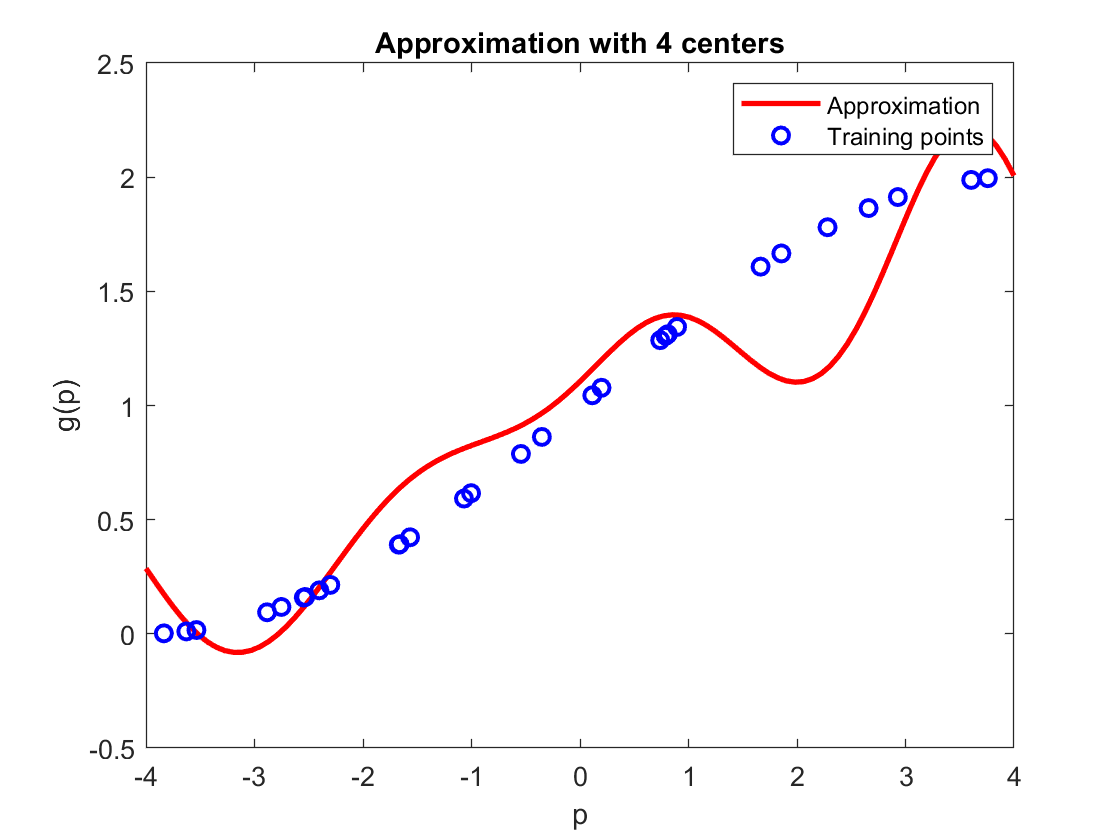
\includegraphics[width=0.4\textwidth]{Problem2_4_random.png}
	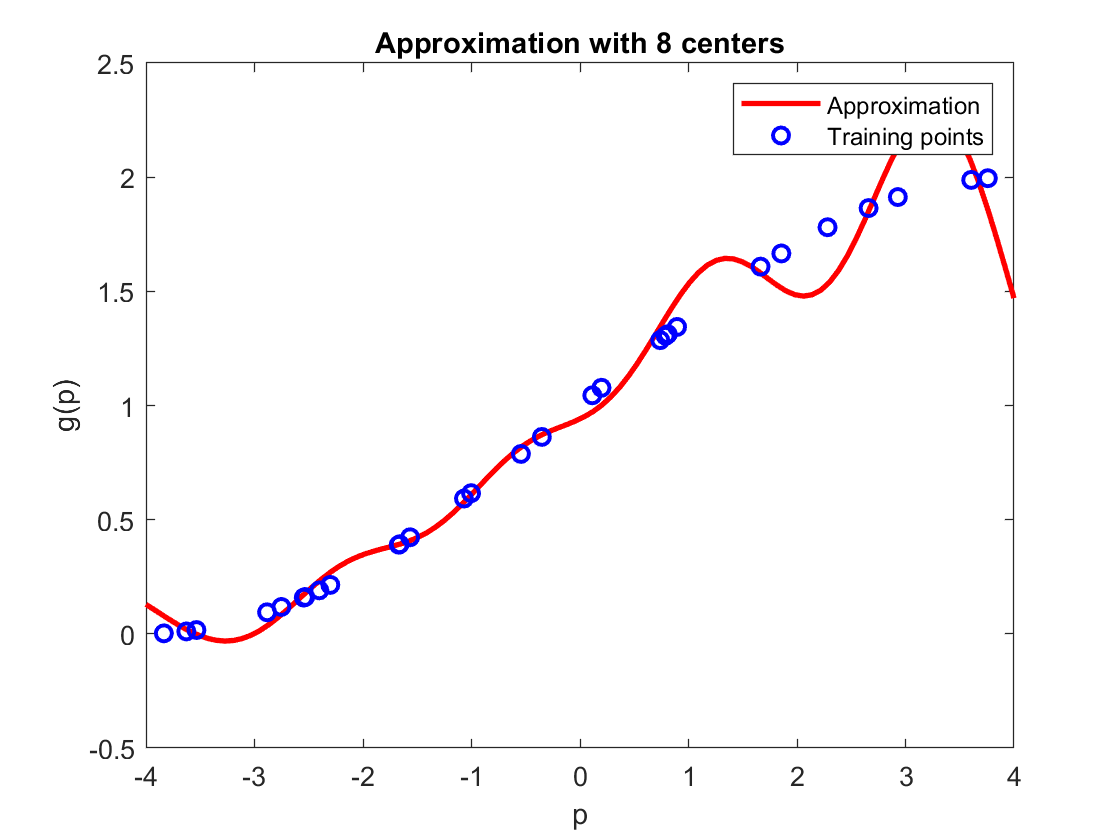
\includegraphics[width=0.4\textwidth]{Problem2_8_random.png} \\
	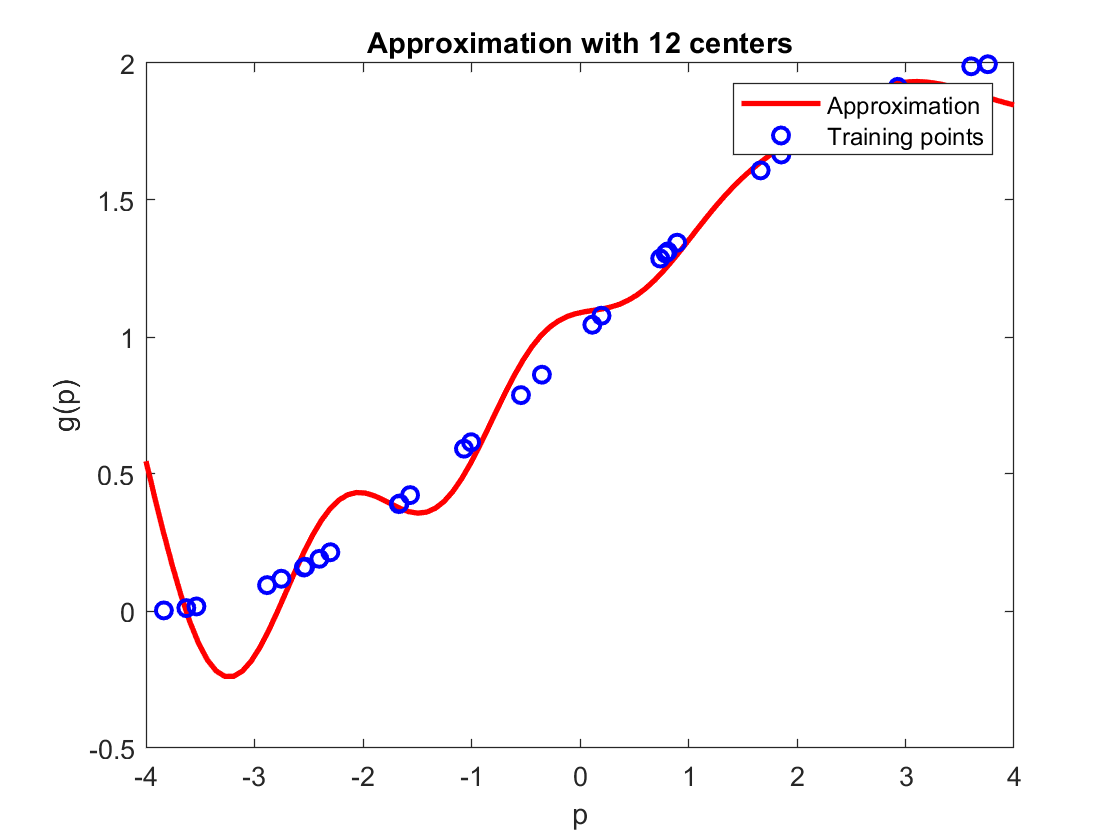
\includegraphics[width=0.4\textwidth]{Problem2_12_random.png}
	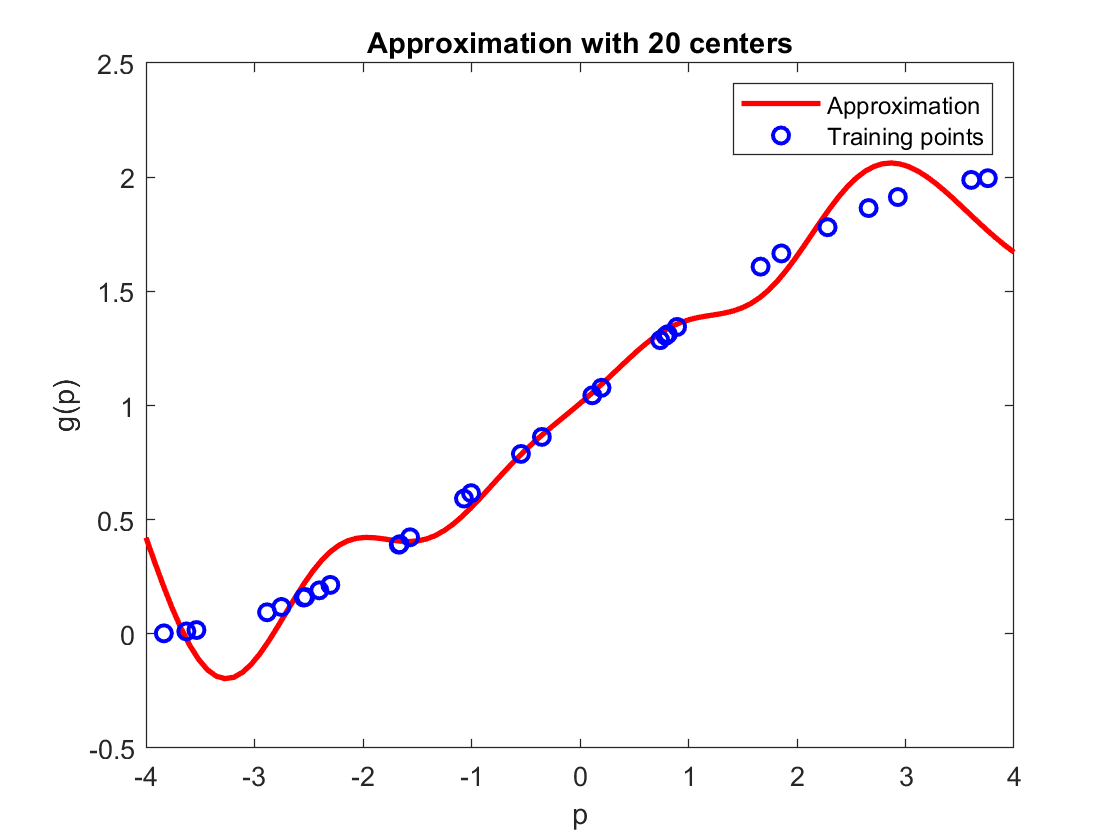
\includegraphics[width=0.4\textwidth]{Problem2_20_random.png}

	\item Uniform reference points: 
	The sum squared errors for 4,8,12 and 20 centers are 0.48242, 0.048453, 0.17237 and 0.044526 respectively. The plots are: \\
	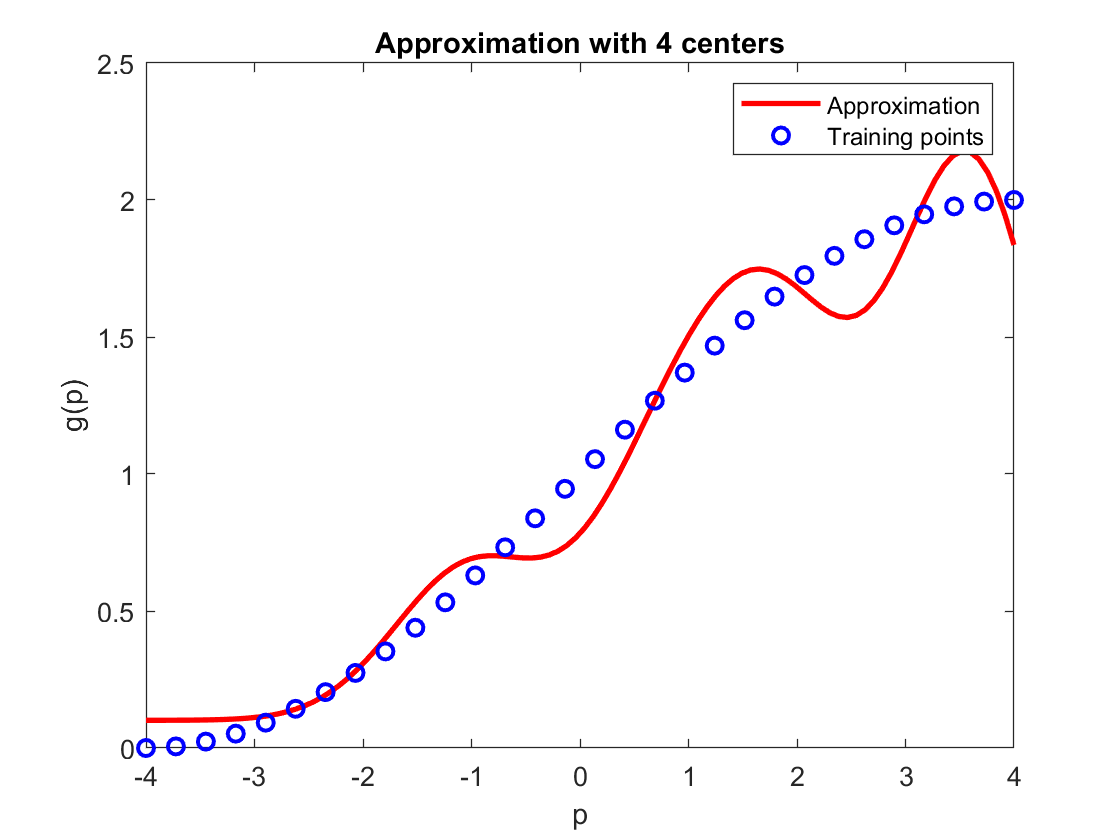
\includegraphics[width=0.4\textwidth]{Problem2_4_uniform.png}
	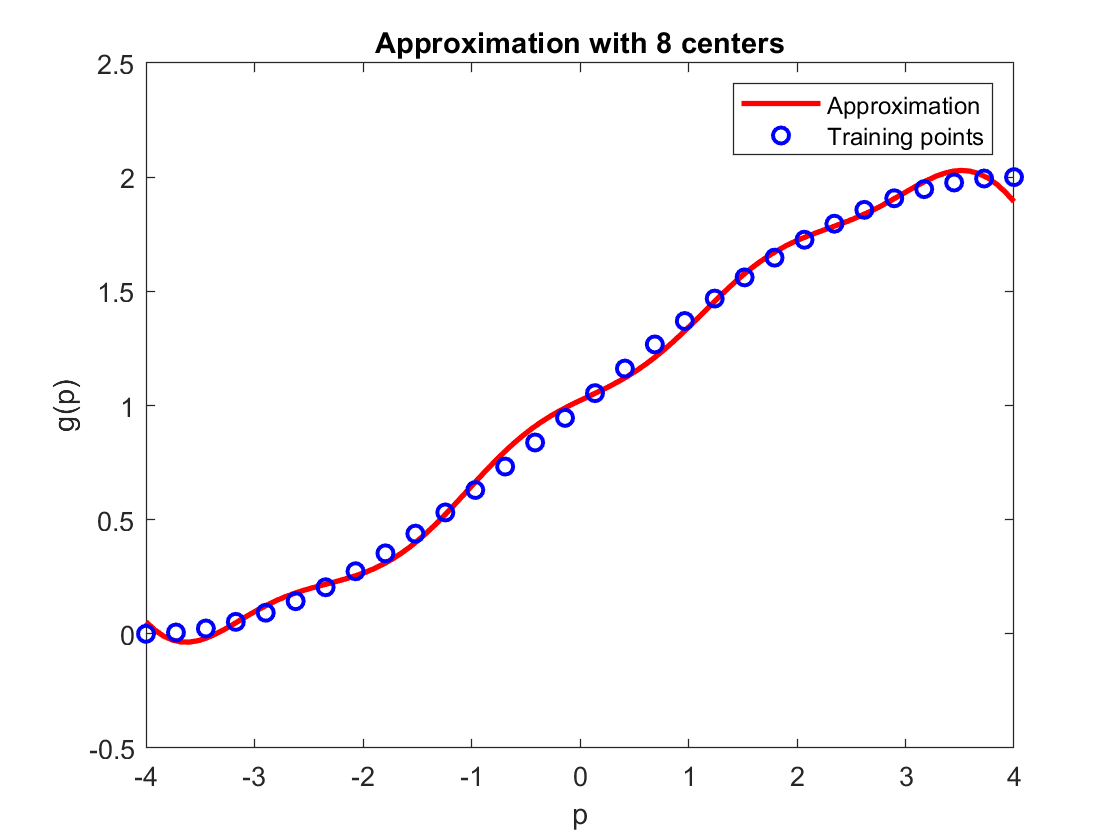
\includegraphics[width=0.4\textwidth]{Problem2_8_uniform.png} \\
	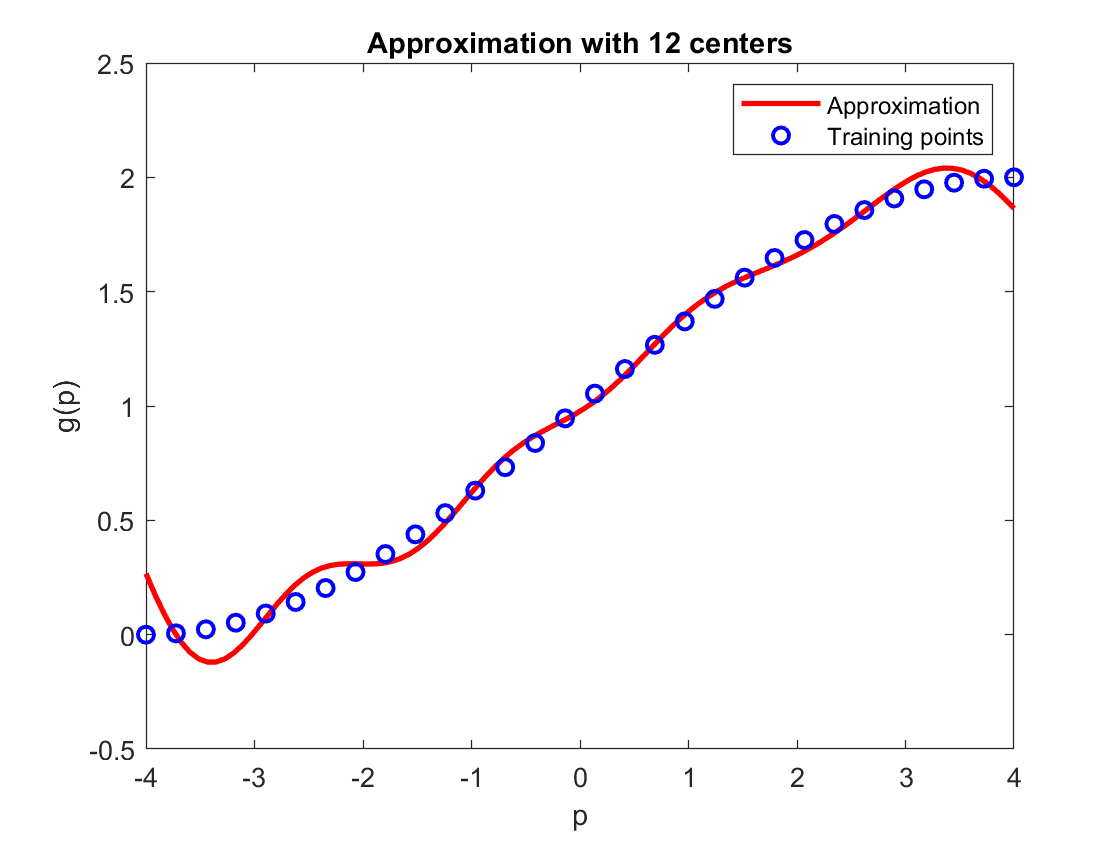
\includegraphics[width=0.4\textwidth]{Problem2_12_uniform.png}
	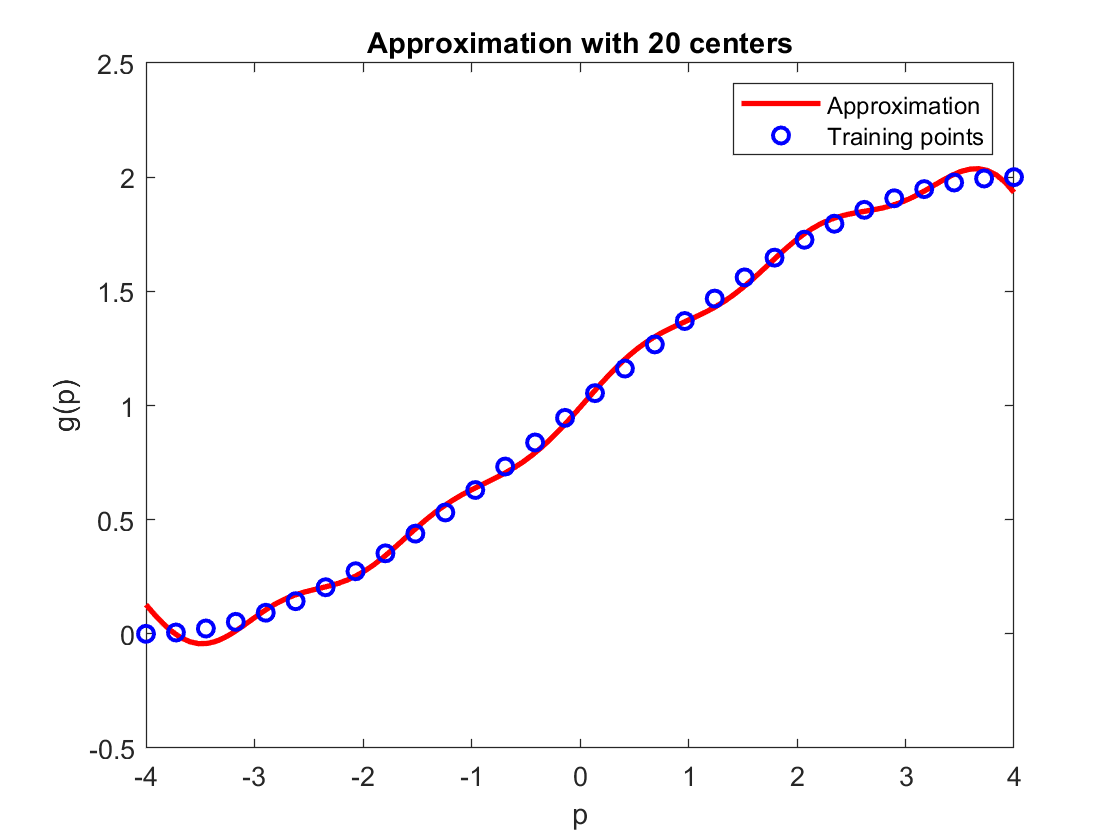
\includegraphics[width=0.4\textwidth]{Problem2_20_uniform.png}
\end{itemize}

We can observe from the errors and the plots that the uniform reference points produce much better results.


%Problem 3
\newpage
\noindent \textbf{Problem 3}

\noindent The net input expression for LVQ networks calculates the distance between the input 
and each weight vector directly, instead of using the inner product. The result is that the 
LVQ network does not require normalized input vectors. This technique can also be 
used to allow a competitive layer to classify non-normalized vectors. Such a network is 
shown in figure below.

\begin{center}
    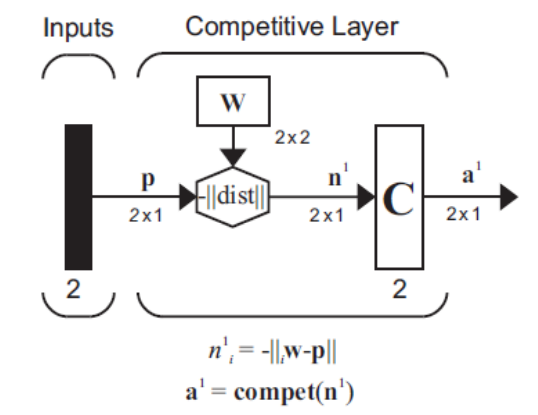
\includegraphics[width=0.4\textwidth]{pr3.png}
\end{center}

\noindent Use this technique to train a two-neuron competitive layer on the (non-normalized) 
vectors below, using a learning rate, $\alpha$, of 0.5 

\begin{center}
    $p_1 = \begin{bmatrix}
        1\\
        1
      \end{bmatrix}, p_2 = \begin{bmatrix}
        -1\\
        2
      \end{bmatrix}, p_3 = \begin{bmatrix}
        -2 \\
        2
      \end{bmatrix}$
\end{center}

\noindent Present the vectors in the following order: $p_1, p_2, p_3, p_2, p_3, p_1$. 
Here are the initial weights of the network: 

\begin{center}
    $w_1 = \begin{bmatrix}
        0\\
        1
      \end{bmatrix}, w_2 = \begin{bmatrix}
        1\\
        0
      \end{bmatrix}$
      \vspace{1cm}
\end{center}

\noindent \underline{\textbf{\textit{Solution:}}}

\noindent Presenting the vectors in the given order we get: \\\\ \underline{$p_1$:} \\\\$n_1^1 = -||w_1(0)-p_1|| = -1$ and $n_2^1 = -||w_2(0)-p_1|| = -1$ \\\\
$n_1^1 = n_2^1$, so $i^{*} = 1$ and $\alpha = \begin{bmatrix}
  1\\ 
  0
\end{bmatrix}$ \\\\ $w_1(1)=w_1(0) - \alpha(p_1-w_1(0)) = \begin{bmatrix}
  0 \\
  1
\end{bmatrix} + 0.5 (\begin{bmatrix}
  1\\
  1
\end{bmatrix} - \begin{bmatrix}
  0\\
  1
\end{bmatrix}) =  \begin{bmatrix}
  0.5\\
  1
\end{bmatrix}$
\\\\ \underline{$p_2$:} \\\\$n_1^2 = -||w_1(1)-p_2|| \approx -1.803$ and $n_2^2 = -||w_2(1)-p_2|| approx -2.829$ \\\\
$n_1^2 > n_2^2$, so $i^{*} = 1$ and $\alpha = \begin{bmatrix}
  0\\ 
  1
\end{bmatrix}$ \\\\ $w_2(1)=w_2(0) - \alpha(p_2-w_2(0)) = \begin{bmatrix}
  1 \\
  0
\end{bmatrix} - 0.5 (\begin{bmatrix}
  -1\\
  2
\end{bmatrix} - \begin{bmatrix}
  1\\
  0
\end{bmatrix}) =  \begin{bmatrix}
  2\\
  -1
\end{bmatrix}$
\newpage
\noindent\underline{$p_3$:} \\\\$n_1^3 = -||w_1(2)-p_3|| = -70$ and $n_2^3 = -||w_2(2)-p_3|| = -5$ \\\\
$n_1^3 > n_2^3$, so $i^{*} = 1$ and $\alpha = \begin{bmatrix}
  1\\ 
  0
\end{bmatrix}$ \\\\ $w_1(2)=w_1(1) - \alpha(p_3-w_1(1)) = \begin{bmatrix}
  0.5 \\
  1
\end{bmatrix} - 0.5 (\begin{bmatrix}
  -2\\
  2
\end{bmatrix} - \begin{bmatrix}
  0.5\\
  1
\end{bmatrix}) =  \begin{bmatrix}
  1.75\\
  0.5
\end{bmatrix}$
\\\\ \underline{$p_2$:} \\\\$n_1^4 = -||w_1(3)-p_2|| -3.13$ and $n_2^4 = -||w_2(3)-p_2|| \approx -4.24$ \\\\
$n_1^4 > n_2^4$, so $i^{*} = 1$ and $\alpha = \begin{bmatrix}
  1\\ 
  0
\end{bmatrix}$ \\\\ $w_1(3)=w_1(2) - \alpha(p_2-w_1(2)) = \begin{bmatrix}
  1.75 \\
  0.5
\end{bmatrix} - 0.5 (\begin{bmatrix}
  -1\\
  2
\end{bmatrix} - \begin{bmatrix}
  1.75\\
  0.5
\end{bmatrix}) =  \begin{bmatrix}
  0.375\\
  1.25
\end{bmatrix}$
\\\\\underline{$p_3$:} \\\\$n_1^5 = -||w_1(4)-p_3|| = -2.95$ and $n_2^5 = -||w_2(4)-p_3|| = -5$ \\\\
$n_2^5 > n_1^5$, so $i^{*} = 2$ and $\alpha = \begin{bmatrix}
  1\\ 
  0
\end{bmatrix}$ \\\\ $w_1(4)=w_1(3) - \alpha(p_3-w_1(3)) = \begin{bmatrix}
  0.375 \\
  1.25
\end{bmatrix} - 0.5 (\begin{bmatrix}
  -2\\
  2
\end{bmatrix} - \begin{bmatrix}
  0.375\\
  1.25
\end{bmatrix}) =  \begin{bmatrix}
  1.5625\\
  0.875
\end{bmatrix}$
\\\\ \underline{$p_1$:} \\\\$n_1^6 = -||w_1(5)-p_1|| = -0.57$ and $n_2^6 = -||w_2(5)-p_1|| = -2.23$ \\\\
$n_1^6 > n_2^6$, so $i^{*} = 1$ and $\alpha = \begin{bmatrix}
  1\\ 
  0
\end{bmatrix}$ \\\\ $w_1(5)=w_1(4) - \alpha(p_1-w_1(4)) = \begin{bmatrix}
  1.5625 \\
  0.875
\end{bmatrix} - 0.5 (\begin{bmatrix}
  1\\
  1
\end{bmatrix} - \begin{bmatrix}
  1.5625 \\
  0.875
\end{bmatrix}) \approx  \begin{bmatrix}
  1.28\\
  0.94
\end{bmatrix}$




%Problem 7
\newpage
\noindent \textbf{Problem 7}

\noindent Model the following expressions as fuzzy subsets:
\begin{enumerate} [label = \Alph*]
    \item Large integers.
    \item Very small numbers.
    \item Medium-weight men.
    \item Numbers approximately between 10 and 20.
\end{enumerate}

\vspace{1cm}

\noindent \underline{\textbf{\textit{Solution:}}}\\
\begin{enumerate} [label = \Alph*]
  \item $\mu_{\utilde{A}}(x) = \begin{cases}
    0 &\text{for } x \leq 100 \\
    \frac{1}{1+\frac{1}{(x-100)^2}} &\text{for } x>100\\
    
  \end{cases}$, assuming that a large integer is an integer bigger than 100.\\\\
  \item $\mu_{\utilde{B}}(x) = \begin{cases}
    1 &\text{for } x \leq 0 \\
    \frac{1}{1+\frac{1}{(x-0.0001)^2}} &\text{for } x>100\\
  \end{cases}$ \\ \\
  \item $\mu_{\utilde{C}}(x) = 
    \frac{1}{1+\frac{1}{(x-75)^2}}$, assuming that a medium-weight man weights 75kg.\\\\
  \item $\mu_{\utilde{D}}(x) = \begin{cases}
    \frac{x^2}{100} & \text{for } x<10 \\
    1 &\text{for } 10 \leq x \leq 20 \\
    \frac{(x-30)^2}{100} &\text{for } x>20\\
    
  \end{cases}$,
\end{enumerate}


%Problem 8
\newpage
\noindent \textbf{Problem 8}

\noindent During the lectures, we have defined the concept of ordinary subset of level $\alpha$ of a fuzzy 
subset. The analogous definition, i.e., the ordinary relation of level $\alpha$ of a fuzzy relation, is 
straightforward. Determine analytically and show graphically the ordinary relation of level 
0.3 for the fuzzy relation with membership function: $\mu_{\utilde{R}}(x, y) = 1 - 1/(1+x^2+y^2)$.
\\ \\
\noindent \underline{\textbf{\textit{Solution:}}}

\noindent Analytically we need to solve: \\
$1-1/(1+x^2+y^2) \geq 0.3 $ \\ $\rightarrow 1+x^2+y^2 \geq 1/0.7 $ \\
$ \rightarrow x^2 + y^2 \geq 3/7$
\\ \\
\noindent Graphically we get the following plot:

\begin{center}
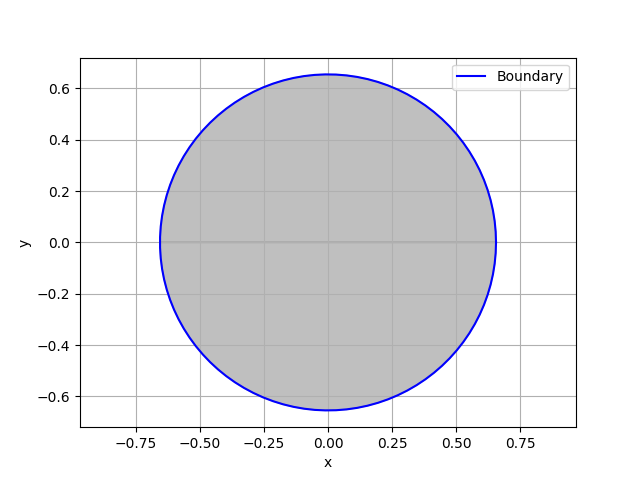
\includegraphics[width=0.6\textwidth]{Problem8.png}
\end{center}


%Problem 9
\newpage
\noindent \textbf{Problem 9}

\noindent Consider the reference set E= $[0, \alpha] \subset R$. If $\utilde{A}$ is the fuzzy subset defined by 
$\mu_{\utilde{A}}(x)$, give the index v of fuzziness of $\utilde{A}$ for:

\begin{enumerate} [label=\Alph*]
  \item $\mu_{\utilde{A}}(x)$ = $x^2/\alpha^2$, $x \in [0, \alpha].$
  \item $\mu_{\utilde{A}}(x) = 4x^2/\alpha^2$ if $0 \leq x\leq \alpha/2$ and $\mu_{\utilde{A}}(x) = 4(x-\alpha)^2/\alpha^2$ if $\alpha/2  <x \leq \alpha$
\end{enumerate}

\vspace{1cm}
\noindent \underline{\textbf{\textit{Solution:}}}

\noindent In order to calculate the index of fuzziness we will use the formula: $\nu = \frac{2}{n} * d(\utilde A,  \bar{ \utilde{ A}})$


\noindent First we will calculate the distance: \\ 
$d(\utilde A,\utilde B) = \sum_{i=1}^{n} | \mu_A(x_i) -  \mu_B(x_i)|$
  $\rightarrow d(\utilde A,\bar{ \utilde{ A}} ) = \sum_{i=1}^{n} | \mu_A(x_i) -  \mu_{\bar{ \utilde{ A}}}(x_i)|$ 
  and $\mu_{\bar{ \utilde{ A}}}(x_i) = 1 - \mu_A(x_i)$ \\
  So $ d(\utilde A,\bar{ \utilde{ A}} ) = \sum_{i=1}^{n} | 2* \mu_A(x_i) -  1| $ \\
\begin{enumerate} [label = \Alph*]
\item
  For the given membership function we get:\\ \\
  $ d(\utilde A,\bar{ \utilde{ A}} ) = \sum_{0}^{a} | 2* \frac{x^2}{a^2} -  1| = 2 $ \\
  So $\nu = \frac{2}{\alpha}* d(\utilde A,\bar{ \utilde{ A}} ) = \frac{4}{a}$

  \item For the given membership functions we get:\\ \\
  $ d1(\utilde A,\bar{ \utilde{ A}} ) = \sum_{0}^{a/2} | 2* \frac{4*x^2}{a^2} -  1| = 8 $ \\
  $ d2(\utilde A,\bar{ \utilde{ A}} ) = \sum_{a/2}^{a} | 2* \frac{4*(x-a)^2}{a^2} -  1| = -2 $ \\
  $ d(\utilde A,\bar{ \utilde{ A}} ) = d1 + d2 = 6 $
  So $\nu = \frac{2}{\alpha}* d(\utilde A,\bar{ \utilde{ A}} ) = \frac{12}{a}$

\end{enumerate}



%Problem 10
\newpage
\noindent \textbf{Problem 10}

\noindent Determine analytically and show graphically the max-min composition of the two fuzzy 
relations $\utilde{R_1}$ and $\utilde{R_2}$ defined by the following membership functions:\\ \\ $\mu_{\utilde{R_1}} = e^{-k(x-y)^2}$, $k \geq 1$
\\ \\ $\mu_{\utilde{R_2}} = e^{-k(y-z)^2}$, $k \geq 1$

\vspace{1cm}
\noindent \underline{\textbf{\textit{Solution:}}}\\
\noindent The max-min composition of the two relations is: \\ \\
$\mu_{composition}(x,z) = max_y(min(e^{-k(x-y)^2}, e^{-k(y-z)^2}))$. \\ \\ \\Let's first analyze the inner part: $min(e^{-k(x-y)^2}, e^{-k(y-z)^2})$ \\ \\
In order to find the minimum we need to compare the two terms: \\ \\
$e^{-k(x-y)^2} = e^{-k(y-z)^2} \Rightarrow -k(x-y)^2 = -k(y-z)^2 \Rightarrow (x-y)^2 = (y-z)^2$, ($k \geq 1$) \\ \\
If both sides are if the same sign, then: \\ $x-y = y-z \Rightarrow y = \frac{x+z}{2}$.\\\\
If they are of different sign, then: \\ $x-y = z-y \Rightarrow x = z$.\\\\\\Now, we need to evaluate $min(e^{-k(x-y)^2}, e^{-k(y-z)^2})$ at these points: \\ \\
If $\bm{y = \frac{x+z}{2}}$, then $min(e^{-k(x-y)^2}, e^{-k(y-z)^2}) = e^{-k(x-\frac{x+z}{2})^2} = e^{-k\frac{(x-z)^2}{4}}$ \\ \\
If $\bm{x=z}$, then  $min(e^{-k(x-y)^2}, e^{-k(y-z)^2}) = e^{-k(z-y)^2}$. \\\\ So, $\mu_{composition}(x,z) = max(e^{-k\frac{(x-z)^2}{4}},  e^{-k(z-y)^2})$

\end{document}